\documentclass[fleqn]{article} 
\usepackage[a3paper,landscape,vmargin=1.0cm,hmargin=1.5cm]{geometry} 

\usepackage{latexsym}
\usepackage{graphicx}
\usepackage{latexsym}

\usepackage{multicol}

\usepackage{epsfig}
\usepackage[dvips,xdvi]{color}

\usepackage{amsmath}
\usepackage{amssymb}

%--------------------------------------------------------------
	\setlength{\textwidth}{1120pt}
	\setlength{\textheight}{790pt}
%--------------------------------------------------------------
	\setlength{\oddsidemargin}{-50pt}
	\setlength{\evensidemargin}{-50pt}
%--------------------------------------------------------------
	\setlength{\topmargin}{-70pt}
	\setlength{\headheight}{0pt}
	\setlength{\topskip}{0pt}
%--------------------------------------------------------------
	\setlength{\columnseprule}{0.5pt}
	\setlength{\columnsep}{10pt}
%--------------------------------------------------------------
	\renewcommand{\baselinestretch}{1}
%--------------------------------------------------------------
	\setlength{\mathindent}{0.5cm}
	\setlength{\parindent}{7pt}
%--------------------------------------------------------------
	\renewcommand{\bottomfraction}{0.99}
	\renewcommand{\topfraction}{0.99}
	\renewcommand{\textfraction}{0.01}
%--------------------------------------------------------------
	\pagestyle{empty}
%--------------------------------------------------------------


%----------------------------------------------------------------
%	definition
%----------------------------------------------------------------
%----------------------------------------------------------------
%   equation 環境
%----------------------------------------------------------------
%		\def\topmat{\ \\ \vspace{-4mm}}
%		\def\botmat{\ \\ \vspace{-2mm}}
%		\def\bes{\vspace*{2mm}}
%		\def\ees{\ \\[-2mm]}
	%........................................................
	% equationの環境設定(\be,\ee)
	%      例 \bea 式 & 式 & 式 \nonumber\\ 式 & 式 & 式 \eea
	%........................................................
%		\def\be{\\ \ \\[-12mm] \begin{equation}}
%		\def\ee{\end{equation} \ \\[-11mm]}
		\newcommand{\be}{\begin{equation}}
		\newcommand{\ee}{\end{equation}}
	%........................................................
	% eqnarrayの環境設定(\bea,\eea)
	%      例 \bea 式 & 式 & 式 \nonumber\\ 式 & 式 & 式 \eea
	%........................................................
%		\def\bea{\\ \ \\[-16mm] \begin{eqnarray}}
%		\def\eea{\end{eqnarray} \ \\[-13mm]}
		\newcommand{\bea}{\begin{eqnarray}}
		\newcommand{\eea}{\end{eqnarray}}
	%........................................................
	% 番号なしeqnの環境設定(\nbe,\nee)
	%      例 \nbe 式 \\ 式  \nee
	%........................................................
%		\def\nbe{\\ \ \\[-12mm] \[}
%		\def\nee{\] \ \\[-11mm]}
		\newcommand{\nbe}{\[}
		\newcommand{\nee}{\]}
	%........................................................
	% matrixの入力(\bmatrix,\ematrix)
	%	例 \bmatrix{cc} 1&2\\3&4 \ematrix
	%........................................................
		\renewcommand{\bmatrix}{\left[\begin{array}}
		\newcommand{\ematrix}{\end{array}\right]}
	%........................................................
	% Greek character
	%........................................................
		\def\gggm{\mu}
		\def\ggge{\varepsilon}
		\def\gggw{\omega}
		\def\gggh{\theta}
		\def\ggga{\alpha}
		\def\gggb{\beta}
		\def\gggc{\gamma}
		\def\gggd{\delta}
		\def\gggp{\phi}
	%........................................................
	% others
	%........................................................
%		\def\half{\frac{1}{2}}
		\def\defeq{\stackrel{\rm def}{=}}


\renewcommand{\baselinestretch}{0.8}



%================================================================
\begin{document}
%================================================================
\rightline{
線形システム制御理論（2023.06.02)
\hspace{3cm}
\underline{学籍番号：　　　　　　　　　　　}
\hspace{1cm}
\underline{氏名：　　　　　　　　　　　　　}
\hspace{2cm}
}
%================================================================
\begin{multicols}{4}
%================================================================
\begin{enumerate}
%================================================================

%================================================================
\item
次の状態方程式
\begin{align}
	\frac{dx}{dt} 
	& =	\bmatrix{rr}
			0 & 1 \\
			2 & 3
		\ematrix
		x
		+
		\bmatrix{c}
			0 \\
			1
		\ematrix
		u 
\nonumber
\end{align}
に対して次の状態フィードバックを考える．
\begin{align}
	u & = \bmatrix{cc} f_1 & f_2 \ematrix x
\nonumber
\end{align}

以下の問に答えよ．
\begin{enumerate}
\item
閉ループ系の状態方程式を示せ．
\vspace{6cm}

\item
閉ループ系の状態方程式の特性多項式を求めよ．
\vspace{6cm}

\item
閉ループ系の極が$-2$, $-3$となる状態フィードバックを求めよ．
\vspace{9cm}

\end{enumerate}
%================================================================
\vfill\null
\columnbreak
%================================================================






%================================================================
\item
次のシステムに対してオブザーバを設計したい．
\begin{align}
	\frac{dx}{dt}
	&=	\bmatrix{cc}
			0 & 1 \\
			1 & 2
		\ematrix
		x
		+
		\bmatrix{c}
			1 \\
			2
		\ematrix
		u
\nonumber \\
	y 
	&=	\bmatrix{cc}
			0 & 1 
		\ematrix
		x
\nonumber 
\end{align}

\begin{enumerate}

\item 
オブザーバゲイン$K$の次元に注意してオブザーバの状態方程式を示せ．
\vspace{6cm}

\item
オブザーバの極（推定誤差の収束速さ）が$-1$, $-2$となるようにオブザーバゲイン$K$を求めよ．
\vspace{12cm}

\end{enumerate}
%================================================================
\vfill\null
\columnbreak
%================================================================






%================================================================
\item

図の３質量系を考える．
\begin{center}
　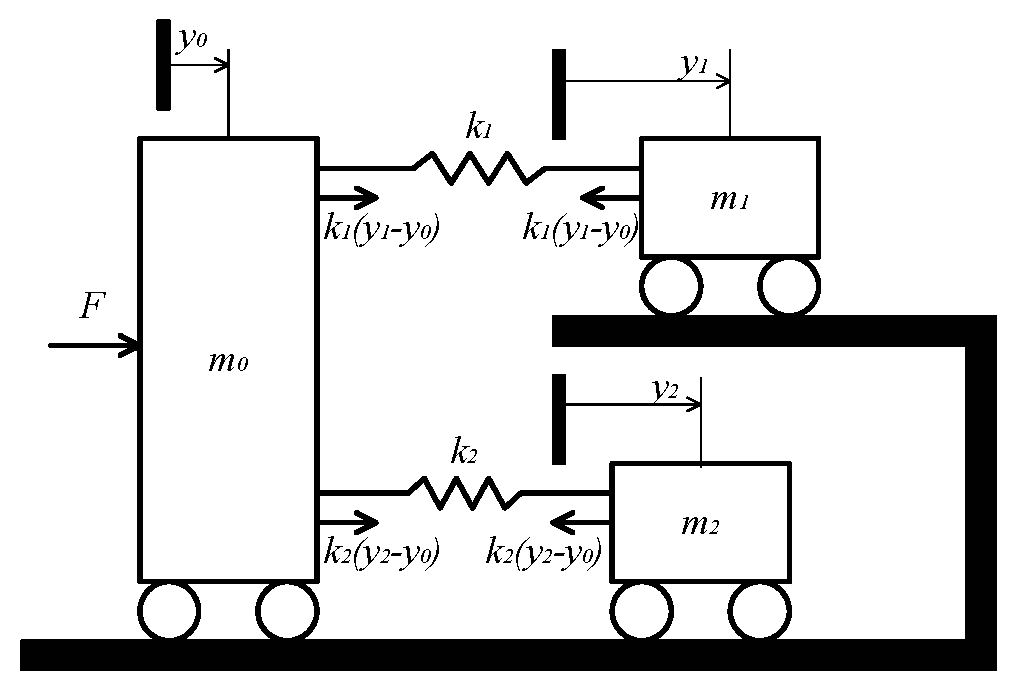
\epsfig{file=car3.eps,scale=0.4}
\end{center}

この３質量系の状態方程式は
{\footnotesize
\begin{align*} 
\hspace*{-10mm}
 \frac{d}{dt} \left(\begin{array}{c}
	         y_0 \\
		     y_1 \\
		     y_2 \\
		     \frac{dy_0}{dt} \\
		     \frac{dy_1}{dt} \\
		     \frac{dy_2}{dt}
		    \end{array}\right)
 =&
 \left(\begin{array}{cccccc}
        0 & 0 & 0 & 1 & 0 & 0      \\
        0 & 0 & 0 & 0 & 1 & 0      \\
        0 & 0 & 0 & 0 & 0 & 1      \\
	-\frac{k_1}{m_0} -\frac{k_2}{m_0}&  \frac{k_1}{m_0} &  \frac{k_2}{m_0} & 0 & 0 & 0 \\
	 \frac{k_1}{m_1}                & -\frac{k_1}{m_1} &  0               & 0 & 0 & 0 \\
	 \frac{k_2}{m_2}                &  0               & -\frac{k_2}{m_2} & 0 & 0 & 0 
       \end{array}\right)
 \left(\begin{array}{c}
	         y_0 \\
		     y_1 \\
		     y_2 \\
		     \frac{dy_0}{dt} \\
		     \frac{dy_1}{dt} \\
		     \frac{dy_2}{dt}
       \end{array}\right)
\\
 &\hspace*{10mm} +
 \left(\begin{array}{c}
        0 \\
        0 \\
        0 \\
	    \frac{1}{m_0} \\
	    0 \\
	    0 
       \end{array}\right)
        F
\end{align*}
}
となる．以下の問いに答えよ．

\begin{enumerate}
\item 
$(m_0, m_1, m_2, k_1, k_2)=(1,1,2,2,1)$の場合，可制御であるか否かを判断せよ．
\vspace{8cm}
%================================================================
\vfill\null
\columnbreak
%================================================================

\item
$(m_0, m_1, m_2, k_1, k_2)=(1,1,2,1,2)$の場合，可制御であるか否かを判断せよ．
\vspace{8cm}

\end{enumerate}

%================================================================
\item
次のシステムについて以下の問に答えよ．
\begin{align}
	\frac{dx}{dt}
	&=	\bmatrix{cc}
			1 & 1 \\
			0 & \alpha
		\ematrix
		x
		+
		\bmatrix{c}
			1 \\
			1
		\ematrix
		u
\nonumber \\
	y 
	&=	\bmatrix{cc}
			1 & 2 
		\ematrix
		x
\nonumber 
\end{align}

\begin{enumerate}

\item 
システムの伝達関数を求めよ．
\vspace{4cm}

\item
システムが不可観測となる$\alpha$を求めよ．
\vspace{4cm}

\item
不可観測となるときのシステムの伝達関数を求め，このときの伝達関数の特徴を示せ．
\vspace{4cm}

\end{enumerate}






%================================================================
\end{enumerate}
%================================================================
\end{multicols}
%================================================================
\end{document}
%================================================================


